\documentclass[12pt, letterpaper]{article}

\usepackage[margin=1.25in]{geometry}
\usepackage{amsmath, amssymb}
\usepackage{graphicx}
\usepackage{authblk}
\usepackage{indentfirst}
\usepackage{blindtext}
\graphicspath{{./Images/}}
\setlength\parindent{12pt}

\title{STAT131 Week 1 Notes}
\author{William Santosa}
\date{Winter 2022 Quarter}

\begin{document}

\maketitle

\section{Introduction}
This document covers essential information and example problems with answers in Chapter 1 in the "Introduction to Probability, 2nd Edition" written by Joseph K. Blitzstein and Jessica Hwang.

\section{Important Definitions}

Contains important definitions for understanding Chapter 1 in textbook.

\begin{itemize}
    \item \textit{Sample Space S} is the set of all possible outcomes from the experiment
    \item \textit{Event A} is the subset of \emph{sample space} S
    \begin{itemize}
        \item \textbf{Note:} We say an event \textit{occurred} if the actual outcome is in A.
    \end{itemize}
    \item \textit{Complement} of A are the elements not in A, denoted as \[A^{c}\]
    \item \textit{Union} of A and B occurs if \textit{at least one} of A or B occurs \[A \cup B\]
    \item \textit{Intersect} of A and B occurs if only and if \textit{both} of A and B occur \[A \cap B\]
    \item \textit{De Morgan's laws} are a pair of transformation rules vital to set theory \[(A\cup B)^{c} = A^{c}\cap B^{c}\] \begin{center} and \end{center}\[(A\cap B)^{c} = A^{c}\cup B^{c}\]
\end{itemize}

\section{Screenshots}
\begin{enumerate}
    \item 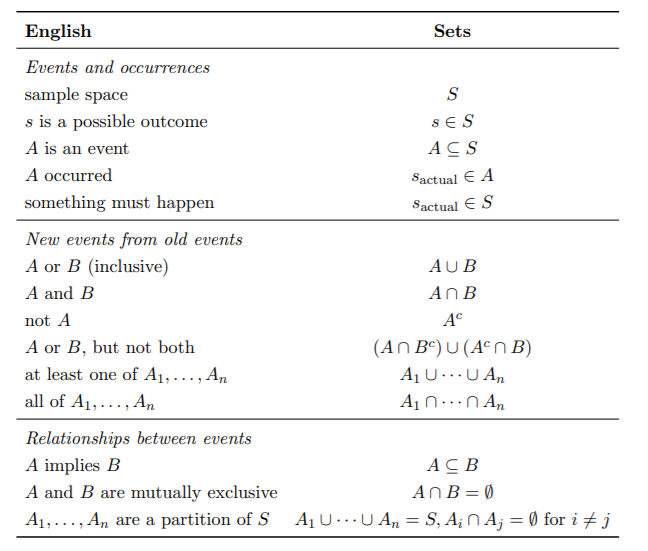
\includegraphics{English.png}
\end{enumerate}

\end{document}